\newpage
\section{Graphic Matroids}\label{sec:graphic-matroids}


First, we are not just interested in simple graphs. For reminder, a simple graph $G$ is an ordered pair $G = (V, E)$ where $V$ is a finite set (of vertices) and $E$ is a collection of two-element subsets of $V$ (of edges). We will extend the notion of edge to include \textit{loops} and \textit{parallel edges}. For this, we will illustrate the two notions. Intuitively, a loop is an edge going from a vertex to itself, and one can also have multiple loops on a single vertex. Parallel edges are intuitively multiple edges between the same vertices.


%For example, in figure \ref{ilustratinloops}, we have a vertex $a$ with a single loop and vertex $d$ with 3 loops.

\begin{figure}[H]
    \centering
    \subfloat[\centering Loops]{
    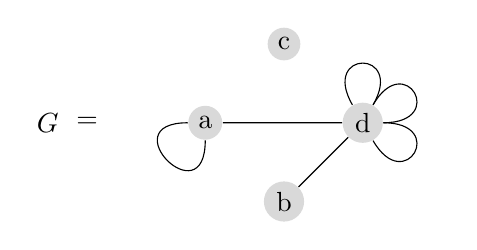
\begin{tikzpicture}[every loop/.style={}]

  \tikzstyle{vertex}=[circle,fill=black!15,minimum size=8pt,inner sep=2pt]

  \node (name) at (-2,0) {$G $};
  \node (another name) at (-1.5,0) {$ =$};
   
  
  \node[vertex] (v2) at (0,0)   {a};
  \node[vertex] (v3) at (1,-1)  {b};
  \node[vertex] (v4) at (1,1)  {c};
  \node[vertex] (v5) at (2,0)  {d};
  \draw (v2) edge[in=270,out=180, loop] node[below] {} ();

  \draw (v5) edge[in=300,out=0, loop] node[below] {} ();
  \draw (v5) edge[in=0,out=60, loop] node[below] {} ();
  \draw (v5) edge[in=60,out=120, loop] node[below] {} ();

  \draw (v2) -- (v5) -- (v3) -- cycle;

  
  %\draw[step=1cm,gray,very thin] (-2,-2) grid (4,4);

%\draw (v1) edge[in=270,out=180, loop] node[below] {2} ();

 
  
\end{tikzpicture}
    
    
    }%
    \qquad
    \subfloat[\centering Parallel edges]{
    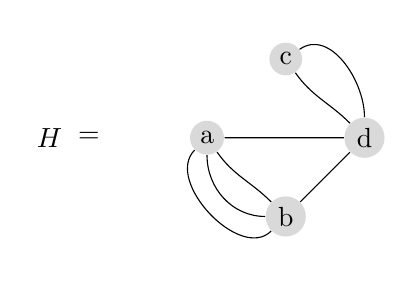
\begin{tikzpicture}[every loop/.style={}]

  \tikzstyle{vertex}=[circle,fill=black!15,minimum size=8pt,inner sep=2pt]

  \node (name) at (-2,0) {$H $};
  \node (another name) at (-1.5,0) {$ =$};
   
  
  \node[vertex] (v2) at (0,0)   {a};
  \node[vertex] (v3) at (1,-1)  {b};
  \node[vertex] (v4) at (1,1)  {c};
  \node[vertex] (v5) at (2,0)  {d};
  
  \draw (v2) edge[in=225,out=225] node[below] {} (v3);
  \draw (v2) edge[in=180,out=270] node[below] {} (v3);
  \draw (v2) edge[in=135,out=305] node[below] {} (v3);

  \draw (v4) edge[in=135,out=305] node[below] {} (v5);
  \draw (v4) edge[in=90,out=35] node[below] {} (v5);


  \draw (v2) -- (v5) -- (v3) -- cycle;

  
 

%\draw (v1) edge[in=270,out=180, loop] node[below] {2} ();

 
  
\end{tikzpicture}
    }%
    \caption{Graph $G$ with loops and graph $H$ with parallel edges}%
    \label{ilustratinloops}%
\end{figure}


In figure \ref{ilustratinloops} we see graphs $G$ and $H$, the first one has loops and the second one has parallel edges. One way to make both constructions formal is to use \textit{multiset} of edges instead of a set, as in \cite[4]{oxley1}.

However, the formal construction of loops and parallel edges is not so important, as we will see in the preceding text, and one can usually restrict its attention to simple graphs. What is important for us is how do the loops and parallel edges interact with the notion of a \textit{cycles} in graphs. 

For clarity, we define exactly what we mean by a cycle in a simple graph.

\begin{defn}
    Let $G = (V,E)$ be a simple graph. Then a sequence $v_0, v_1, \cdots, v_k$ of vertices, where $k\geq 3$, is called a \textit{cycle} if the following condidtions are satisfied
    
    \begin{enumerate}

        \item If $v_i = v_j$ for some $0 \leq i,j \leq k$ then $i = j$ or $k = 0$, in other words $v_0 = v_k$ while all of the other vertices are distinct. 
        
        \item For all $0\leq i < k$, we have that $v_i$ and $v_{i+1}$ are incident.
    \end{enumerate}
\end{defn}

We need to extend the notion of a cycle to non-simple graphs. To do this, we additionally define that a loop is a cycle of length one. Intuitively, this is consistent with the simple graph definition, because our initial and final vertex is the same without any vertices in between. Similarly, we define a set of two distinct parallel edges to be a cycle of length two. This makes sense because the first and the last vertex is the same with one in between, but edges cannot repeat, so we have to go via different edges connecting two vertices.




%In particular, we see that by, we have that if a loop is in a cycle, then the whole cycle consists only of that loop - we have one vertex appearing multiple times in a sequence - the beginning/ending vertex. 

Also, for parallel edges, at most one from a class of parallel edges connecting the same two vertices can appear in a cycle.


\begin{figure}[H]
\centering

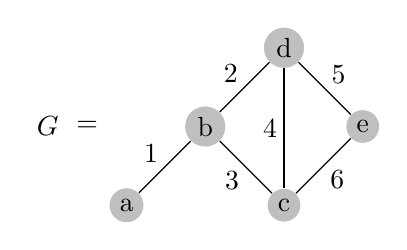
\begin{tikzpicture}[every loop/.style={}]

      \tikzstyle{vertex}=[circle,fill=black!25,minimum size=6pt,inner sep=2pt]

  \node (name) at (-2,0) {$G $};
  \node (another name) at (-1.5,0) {$ =$};
   
  \node[vertex] (v1) at (-1,-1) {a};
  \node[vertex] (v2) at (0,0)   {b};
  \node[vertex] (v3) at (1,-1)  {c};
  \node[vertex] (v4) at (1,1)  {d};
  \node[vertex] (v5) at (2,0)  {e};
  \draw (v1) -- node[midway, xshift=-0.5em, yshift=0.5em]{1} (v2) -- node[midway, xshift=-0.5em, yshift=-0.5em]{3} (v3) -- cycle;
  \draw (v2) -- node[midway, xshift=-0.5em, yshift=0.5em]{2} (v4) -- node[midway, xshift=0.5em, yshift=0.5em]{5} (v5) -- node[midway, xshift=0.5em, yshift=-0.5em]{6} (v3) -- cycle;
  \draw (v4) -- node[midway, xshift=-0.5em, yshift=0em]{4} (v3);

  
  %\draw[step=1cm,gray,very thin] (-2,-2) grid (4,4);

%\draw (v1) edge[in=270,out=180, loop] node[below] {2} ();

 
  
\end{tikzpicture}
\caption{Simple graph on 6 edges}
  \label{simp}

\end{figure}

We consider a concrete example of a simple graph and build a matroid out of it. Let us label the set of edges $E = \{1, 2, 3, \cdots, 6\}$. We will define a collection of subsets $\mathcal{C}$ of $E$ where $C \in \mathcal{C}$ if and only if the set of edges of $C$ forms a cycle in $G$. We check that 

    $$\mathcal{C} = \{\{2,3,4\}, \{4,5,6\}, \{2, 3, 5, 6\}\}.$$

Not surprisingly, the set $E$ with the collection $\mathcal{C}$ being as its set of circuits is, in fact, a matroid. We can check that $\emptyset$ is not in $\mathcal{C}$, none of its members is properly contained in another, and finally 'circuit elimination axiom' works for all three possibilities of taking pairs of elements of $\mathcal{C}$. We will now prove that this works for a general graph.
%``stuff"

\begin{theorem}\label{graphicproof}
Let $G = (V, E)$ be a graph and let $\mathcal{C}$ be the collection of all sets of edges of cycles in $G$. Then $M$ with the ground set $E$ (the set of edges) is matroid with $\mathcal{C}$ as collection of circuits. In particular, if $C_1$, $C_2$ are distinct sets of edges of cycles  and $e \in C_1 \cap C_2 $ then there exists a set of edges of cycle $C_3$ such that $C_3 \subset C_1 \cap C_2 -e$.
\end{theorem}


\begin{proof}

To show that the set $E$ is a matroid with the collection $\mathcal{C}$ of cycles as circuits we have to verify the three circuit axioms. 

\begin{enumerate}

\item[(C1)] The empty set is by our definition not a cycle. For reminder, by our definition a cycle always includes a nonempty set of vertices it is build upon. If it is in a simple graph, then it has to have at least three vertices. Our extended notion also includes loops and parallel edges, which are still built upon at least one vertex. 

\item[(C2)] To show the second property, suppose we have two sets of edges of cycles such that $C_1 \subseteq C_2$ and assume for contradiction there is some $e \in C_2 - C_1$. Then (we are assuming neither of the cycles are loops, that case is clear, because the only possibility is they are equal) the set of edges $C_2 - e$ corresponds to a path from the vertices which $e$ connects. However, there is a cycle $C_1 \subseteq C_2 -e$ which is a subset of a path - a contradiction. So if $C_1 \subseteq C_2$ then $C_2 - C_1$ is empty, in particular then $C_2 = C_1$ and all three circuit axioms are satisfied.



    
   \item[(C3)] Finally, we prove the third property. Let $C_1$ and $C_2$ be two cycles. We would like to show that there is a set of edges of cycle $C_3 \subset C_1 \cap C_2 - e$ for any $e \in C_1 \cap C_2$.
 

   \begin{figure}[h] 
\caption{A graph of suspicious shape, having three cycles.}
\label{impostor2}
\begin{subfigure}[h]{0.245\textwidth}
  \caption{Graph}
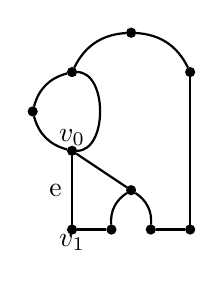
\begin{tikzpicture}[node distance={10mm}, thick, main/.style = {draw,circle,fill,inner sep=1pt}] 
  \node[main] (1) at (0,0) {}; 
  \node[main] (3) at (-0.5,0.5) {}; 
  \node[main] (4) at (0, 1) {}; 
  \node[main] (5) at (0, -1) {}; 
  \node[main] (6) at (1.5, -1) {}; 
  \node[main] (7) at (0.75, 1.5) {}; 
  \node[main] (8) at (1.5, 1) {}; 
  \node[main] (9) at (0.5, -1) {}; 
  \node[main] (10) at (1, -1) {}; 
  \node[main] (11) at (0.75, -0.5) {}; 
  \draw (1) to [bend left] (3);
  \draw (1) to [bend right=90] (4) ;
  \draw (3) to [bend left] (4);
  \draw (4) to [bend left] (7);
  \draw (7) to [bend left] (8);
  \draw (8) to (6);
  \draw (5) to (9);
  \draw (6) to (10);
  \draw (9) to [bend left] (11);
  \draw (10) to [bend right] (11);
  \draw (1) to node[midway,left] {e} node[above,pos=0] {$v_0$} node[below,pos=1] {$v_1$} (5);
  \draw (1) to (11);
  \end{tikzpicture} 
\end{subfigure}
\begin{subfigure}[h]{0.245\textwidth}
  \caption{$C _1$}
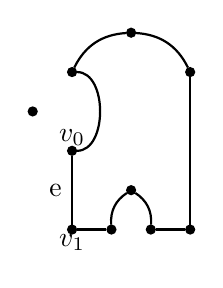
\begin{tikzpicture}[node distance={10mm}, thick, main/.style = {draw,circle,fill,inner sep=1pt}] 
  \node[main] (1) at (0,0) {}; 
  \node[main] (3) at (-0.5,0.5) {}; 
  \node[main] (4) at (0, 1) {}; 
  \node[main] (5) at (0, -1) {}; 
  \node[main] (6) at (1.5, -1) {}; 
  \node[main] (7) at (0.75, 1.5) {}; 
  \node[main] (8) at (1.5, 1) {}; 
  \node[main] (9) at (0.5, -1) {}; 
  \node[main] (10) at (1, -1) {}; 
  \node[main] (11) at (0.75, -0.5) {}; 
  \draw (1) to [bend right=90] (4);
  \draw (4) to [bend left] (7);
  \draw (7) to [bend left] (8);
  \draw (8) to (6);
  \draw (5) to (9);
  \draw (6) to (10);
  \draw (9) to [bend left] (11);
  \draw (10) to [bend right] (11);
  \draw (1) to node[midway,left] {e} node[above,pos=0] {$v_0$} node[below,pos=1] {$v_1$} (5);
\end{tikzpicture} 
\end{subfigure}
\begin{subfigure}[h]{0.245\textwidth}
  \caption{$C _2$}
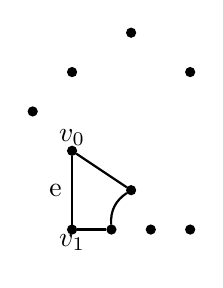
\begin{tikzpicture}[node distance={10mm}, thick, main/.style = {draw,circle,fill,inner sep=1pt}] 
  \node[main] (1) at (0,0) {}; 
  \node[main] (3) at (-0.5,0.5) {}; 
  \node[main] (4) at (0, 1) {}; 
  \node[main] (5) at (0, -1) {}; 
  \node[main] (6) at (1.5, -1) {}; 
  \node[main] (7) at (0.75, 1.5) {}; 
  \node[main] (8) at (1.5, 1) {}; 
  \node[main] (9) at (0.5, -1) {}; 
  \node[main] (10) at (1, -1) {}; 
  \node[main] (11) at (0.75, -0.5) {}; 
  \draw (1) to node[midway,left] {e} node[above,pos=0] {$v_0$} node[below,pos=1] {$v_1$} (5);
  \draw (1) to (11);
  \draw (5) to (9);
  \draw (9) to [bend left] (11);
\end{tikzpicture} 
\end{subfigure}
\begin{subfigure}[h]{0.245\textwidth}
  \caption{$C _3$} 
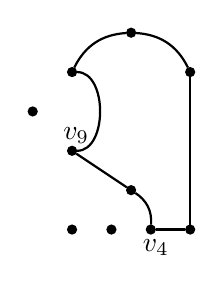
\begin{tikzpicture}[node distance={10mm}, thick, main/.style = {draw,circle,fill,inner sep=1pt}] 
  \node[main] (1) at (0,0) {}; 
  \node[main] (3) at (-0.5,0.5) {}; 
  \node[main] (4) at (0, 1) {}; 
  \node[main] (5) at (0, -1) {}; 
  \node[main] (6) at (1.5, -1) {}; 
  \node[main] (7) at (0.75, 1.5) {}; 
  \node[main] (8) at (1.5, 1) {}; 
  \node[main] (9) at (0.5, -1) {}; 
  \node[main] (10) at (1, -1) {}; 
  \node[main] (11) at (0.75, -0.5) {}; 
  \draw (1) to [bend right=90] (4);
  \draw (4) to [bend left] (7);
  \draw (7) to [bend left] (8);
  \draw (8) to (6);
  \draw (6) to node[below,pos=1] {$v_4$} (10);
  \draw (10) to [bend right] (11);
  \draw (1) to node[above,pos=0] {$v_9$} (11);
\end{tikzpicture} 
\end{subfigure}
    \end{figure}

    First, if $C_1 \cap C_2 = \emptyset$ there is nothing to prove, because the conditional part of the if statement in (C3) is not satisfied.
   
   Second, assume there exists $e \in C_1 \cap C_2$. Let the cycle $C_1$ correspond to the sequence of incident vertices  $v_0, \cdots, v_n = v_0$ and let (without loss of generality) the special edge in the intersection be the edge $e = \{v_0, v_1\}$. The idea of the proof is very simple. Our goal is to find a cycle in the set of edges $C_1 \cup C_2 -e$. We go around $C_1$ until we can come to a vertex that is disjoint with $C_2$, then we would like to come back that vertex as quickly as we can by using edges of $C_2$, thus avoiding $e.$

   As an illustration of the procedure we see a graph in figure (\ref{impostor2}). The vertex $v_4$ is the first one not in $C_2$ and $v_9$ is the first one in $C_1$ which is after $v_4$ but is back in $C_2$. The cycle obtained in this procedure is $C_3$ which evidently does not include $e.$


    Let $k$ be the smallest integer $1<k< n$ such that the vertex $v_k$ is not in the cycle $C_2$. We know that such an integer exists because we have already proved (C2), so if $C_1$ and $C_2$ are distinct, then necessarily one is not contained in eachother, which means both $C_2 - C_1$ and $C_1 -C_2$ are nonempty.
    Next, let $l$ be the smallest integer $k <l \leq n$ such that $v_l$ is in $C_2$. We know such an integer exist because $v_n \in C_2$.
    
    Let $v_l, w_{l+1}, w_{l+2},  \cdots, v_{k-1}$ be the path of vertices in the cycle $C_2$ which does not include the edge $e$. We know that such a path exists, because $C_2$ is a cycle, so from any two distinct vertices, in particular $v_{l}$ and $v_{k-1}$ (they are distinct since $k<l$ and it cannot hold that $k-1 = 0$ and $l = n$ since this would imply $k = 1$, which cannot hold) there are two paths going from $v_{l}$ to $v_{k-1}$ including only the vertices of $C_2$ - we pick the one that does not include the edge $e$.
    
    We claim that the cycle consisting of vertices $$v_k, v_{k+1}, \cdots v_l, w_{l+1}, \cdots , v_{k-1}, v_k$$ is the desired one and denote its set of edges by $C_3$. By construction the sequence of vertices $v_k, v_{k+1}, \cdots v_l, w_{l+1}, \cdots , v_{k-1}, v_k$ is a cycle, namely the neighboring vertices are incident and except $v_k$ there is no vertex repeating, because we have chosen $v_{k+1}, v_{l-1}, \cdots v_{l-1}$ to be disjoint from $C_2$, while $v_l, w_{l+1}, \cdots, v_{k-1}$ is a path in $C_2$. Crucially, $e \notin C_3$ because we have chosen path $v_{l}, w_{l+1}, \cdots v_{k-1}$ in $C_2$ to not include the edge $e$ and $v_k, v_{k+1}, \cdots v_l$ does not include it because $e = \{v_n = v_0, v_1\}$ and there is no $v_0$ in our cycle. Finally, all the vertices of $C_3$ are inside the vertices of $C_1$ and $C_2$ by construction so, to conclude, the set $C_3$ has the desired property $C_3 \subseteq (C_1 \cup C_2) - e$.
    
    We have to check the possibility that $e$ might be a loop or a parallel edge as well, the above argument works assuming $G$ is a simple graph. If $e$ is a parallel edge than the above argument does still hold since we only know that there is more than one edge between $v_0$
    and $v_1$ which does not change anything. However, if $e$ is a loop then by our convention, a cycle consisting of a loop can just be that loop and nothing else, heuristically, because it begins and ends at a single vertex. So $C_1 = C_2 = \{e\}$ which is a contradiction, since we have assumed $C_1$ and $C_2$ are distinct.

\end{enumerate}

To conclude, the collection of edges of cycles $\mathcal{C}$ satisfies the circuit axioms (C1), (C2) and (C3), therefore we know the cryptomorphic description of matroids in terms of circuits that $E$ is in fact a matroid with having $\mathcal{C}$ as its collection of circuits.

\end{proof}


%\begin{remark}
  %  We also came up with an alternative proof of (C3) for simple graphs in theorem (\ref{graphicproof}), which is shorter, but is less intuitive than the one used, which merely formulized the notion of 'going around the graph'. 

   % Namely, we know that if $C_1$ and $C_2$ are sets of edges of cycles and if $V_1$ and $V_2$ are their sets of vertices, then we know that $|V_1| = |C_1|$ and $|V_2| = |C_2|$. Because the cycles share an edge (we are assuming we are not in the trivial case $|C_1 \cap C_2| = 0$) then the subgraph induced by the edge set $C_1 \cup C_2 - e$ has $|V_1| + |V_2| - 2$ vertices, we just remove the vertices that $e$ connects.
%\end{remark}

\begin{defn}
    We call a matroid $M$ graphic if it is isomorphic to $(E, \mathcal{I})$ where $E$ is the set of edges of some graph and the set of circuits is given by the set of all edge cycles.
\end{defn}



We thus know that given any graph $G$ we have natural matroid structure on its set of edges, by declaring graph cycles to be circuits. Because we know other equivalent descriptions of matroids it is natural to ask what are the independent sets or bases in the case of graphic matroids. 

Suppose that the set of edges $B$ is a base of a graphic matroid. 
% We know that this means that $B$ is independent (we do not yet know how to spot the independent sets in graphs).      % should we remove this?
Since $B$ is maximally indepenent, adding any element not in $B$ to $B$, i.e. any edge not in $B$ to $B$, we get a \textit{dependent set}, which means it contains a circuit. By our definition, this means that it has to contain an edge cycle. Combining all we see that the set of edges $B$ has the property that it does not contain any cycles, however adding any edge makes a cycle - this is the precisely one of the equivalent characterizations of \textit{spanning forests}. Note that we cannot say spanning trees because the graph might not be connected. 

Any independent set is a subset of some basis, so in graphic matroids the set of edges that is independent has to be a subset of some spanning forest, which means it is just a forest.

As an example, we will show that many matroids shown until now are, in fact, graphic. 

 
\begin{figure}[H]
    \centering
    \subfloat[\centering Matrix $A$]{
        $$
    A = \begin{pmatrix}
        2 & 0 & 2 & 0 \\
        1 & -1 & 0 & 0 \\
        0 & 3 & 3 & 0
        \end{pmatrix}
        $$
    }
    \qquad
    \subfloat[\centering Graph $H$]{
    \begin{tikzpicture}[every loop/.style={}]

  \tikzstyle{vertex}=[circle,fill=black!15,minimum size=8pt,inner sep=2pt]

  \node (name) at (-2,-1.5) {$H $};
  \node (another name) at (-1.5,-1.5) {$ =$};
   
  
  \node[vertex] (v2) at (-1,-2)   {};
  \node[vertex] (v3) at (1,-2)  {};
 
  \node[vertex] (v5) at (0,-1)  {};
  

  \draw (v2) -- node[midway, xshift=0em, yshift=-0.5em]{1} (v3)  -- node[midway, xshift=0.6em, yshift=em]{2} (v5) -- node[midway, xshift=-0.6em, yshift=0em]{3} (v2)  --cycle;
  
  \draw (v5) edge[in=150,out=30, loop] node[above] {4} ();
  
  %\draw[step=1cm,gray,very thin] (-2,-2) grid (4,4);

%\draw (v1) edge[in=270,out=180, loop] node[below] {2} ();

 
  
\end{tikzpicture}
    }%
    \caption{Matroid $M[A]$ is graphic; it is isomorphic to the graphic matroid $G$}%
    \label{graphicmatrix}%
\end{figure}

In figure (\ref{graphicmatrix}) we see that the graph $H$ exactly to corresponds to the vector matroid formed on matrix $A$. Edge 4 is a loop, so a dependent set, corresponding to the fact that the fourth column is a zero vector. Similarly, any two element sets of nonzero vector are independent, corresponding to the fact that any two non-loop edges do not form a cycle in the graph. Finally, any set of three or more edges in dependent, which is easily seen in the graph because we have 3 vertices so the size of a spanning forest is at most 3 - 1 = 2.

